\section{Introduction}
Thus far, the dissertation has focused on perceptual choice. This has allowed for the reconciliation of conflicting findings from other researchers \parencite{spektorWhenGoodLooks2018b,trueblood2013not}, using a Thurstonian choice model which was developed from the ground up in a simplified choice environment.

However, many decision theorists, in particular those who study context effects, are interested in a wide variety of choice environments. For example, the original demonstration of the attraction effect came from the marketing literature \parencite{huberAddingAsymmetricallyDominated1982d}, where participants selected amongst hypothetical consumer products. This chapter generalizes the paradigm and model from Chapter 2 to preferential choice. Participants were presented with sets of consumer stimuli designed by previous researchers to elicit the repulsion effect. In one phase of the experiment, participants provided the selling prices for consumer goods, a measure analogous to the area judgments from Experiment 2. In a second phase of the experiment, they chose their preferred alternative from the same choice sets. The parameters of the Thurstonian choice model (e.g., means, variances, correlations) were estimated from the pricing data. Crucially, the target-decoy correlation $\rho_{TD}$ was quite strong, a conceptual replication of the results of Experiment 2. The Thurstonian model, conditional on the estimated parameters, was then used to make predictions for the choice data. The model was generally successful in making predictions, albeit with some limitations which are discussed. 

\subsection{Expanding the Paradigm to Preferential Choice}

In Experiment 2, participants provided psychophysical judgments, which were used to estimate the parameters of a Thurstonian choice model. This model, conditional on estimated parameters, was then used to make predictions for choices collected from the same set of participants. 

The next step, in developing and testing both the experimental paradigm and the Thurstonian choice model, was to generalize the paradigm to a preferential choice environment. The goal of this study was to further the understanding of context effects, particularly the attraction and repulsion effect, by estimating means and correlations in preferential choice. Context effects have their empirical and theoretical origins in preferential (consumer) choice, so preferential choice provides a natural next step in this research program.

To test this approach in preferential choice, we collected continuous preference ratings from participants in the former of selling prices, a relatively analogous measure to the continuous area judgments collected in Experiment 2. 

In most studies of consumer preference, researchers collect choice data rather than ratings. There are good reasons for doing so. The literature on willingness to pay (WTP; the largest amount a given consumer is willing to pay for a given product) has shown that, when responding to hypothetical survey questions, participants tend to over-estimate their WTP by a sizeable amount \parencite{breidertREVIEWMETHODSMEASURING2006,schmidtAccuratelyMeasuringWillingness2020}, c.f.~\textcite{miller2011should}. Furthermore, WTP estimates may not simply be off by a constant; \textcite{jedidi2002augmenting} asked participants to state the price they would be willing to pay for a series of Compaq and Dell laptops, and, in a separate phase of the study, to indicate whether they would be willing to pay various actual listing prices for each laptop. Comparing the former stated WTP estimates to those estimated from those estimated from the latter choice data, the results showed that the stated WTP values were sizeably higher, on average, than those estimated from choice data. The stated WTP and estimated WTP values were positively correlated, albeit fairly weakly (maximum $r=.43$). Furthermore, the authors fit two demand curves (one for stated WTP and the other for WTP estimated from choice data) to estimate the percentage of respondents willing to pay various prices for a laptop. The curve based on the stated WTP estimates tended to overestimate demand at low prices and simultaneously underestimate demand at high prices.

\textcite{bridges2012consumer} conducted a study comparing WTP methods, asking hearing-loss patients to provide both Likert-scale ratings of the importance of each hearing aid attribute, as well as to complete a series of pairwise choices between hearing aids with varying attributes (a research technique known as conjoint analysis). The researchers then estimated WTP values for each attribute (e.g., how much would the average consumer be willing to pay for good battery life) using logistic regression. The mean estimated WTP values were ordinally related across methdos, though the authors found that the Likert scale method tended to lead to floor and ceiling effects in WTP. 

In a review of the WTP literature, \textcite{breidertREVIEWMETHODSMEASURING2006} strongly recommended that researchers do not attempt to estimate WTP by directly asking consumers to state their price estimates. Other authors have made similar recommendations \textcite{jedidi2009willingness}. \textcite{miller2011should} compared the empirical value of both stated WTP and choice-based conjoint (CBC) analysis to two other approaches: the Becker, DeGroot, and Marschak auction (BDM, \textcite{becker1964measuring}), where participants bid a price for a product and are required to purchase the product if a price drawn from a lottery is no larger than their bid, and the incentive-aligned choice-based conjoint (ICBC) analysis, a more complex method where the participant completes a hypothetical choice, the researcher infers their WTP based on these data, and this value is put through a BDM mechanism. 

Using a cleaning product as the stimulus, the researchers found that all methods overestimated consumers' true WTP (using actual purchase data as the benchmark). BDM showed the smallest bias, followed by ICBC, stated WTP, and CBC. All methods are do reasonably well, however, in predicting actual purchase data, even given the aforementioned biases. The authors argued that when possible, researchers should use methods based on incentive alignment (i.e., BDM and ICBC) to estimate WTP. They do note that for many applications, however, stated WTP may work reasonably well, particularly when resources are limited and incentive-based methods would be difficult to implement.

In a meta-analysis, \textcite{schmidtAccuratelyMeasuringWillingness2020} found that stated WTP methods actually showed less overestimation bias than indirect methods (e.g,. BDM, ICBC, CBC). However, they also found that bias increased with actual prices of products, and that the bias was stronger in within compared to between-participant studies.

There is not a strong consensus on the best way to estimate pricing data from participants, nor do the measurement properties of WTP data appear to be well understood. These concerns, while crucial to applied researchers, are less pertinent to the current study, as the goal is to estimate prices on a relative, rather than absolute, scale. In other words, if participants over (or under) estimate their preferences by a constant, but generally rate higher valued options more highly than lower valued options, it may still be possible to obtain reasonable estimates on the $\rho$ parameters required by the Thurstonian model. The lack of firm understanding on the measurement properties, however, may still limit the current approach. 

Other researchers have studied context effects with ratings measures. \textcite{wedellUsingJudgmentsUnderstand} collected Likert scale attractiveness ratings for attraction effect stimuli, generally finding that the presence of a decoy increased mean ratings for a target option. \textcite{windschitl2004dud} asked participants to judge the likelihood of various events (also on a Likert scale). They found that the presence of a \textit{dud} (highly unlikely) alternative increased participants' ratings of focal options. \textcite{caiWhenAlternativeHypotheses2023} and \textcite{fang2024context} demonstrated similar effects with continuous probability judgments.

To the author's knowledge, however, there has been no research systematically connecting valuations and choices in a single context effects experiment through a Thurstonian choice model. This chapter seeks to fill this gap in the literature while also generalizing Chapter 2 to consumer choice. Pricing data were collected to estimate the multivariate normal parameters $\boldsymbol{\mu}$ and $\boldsymbol{\Sigma}$ for the choice model from Chapter 2 which was then used these to predict consumer choice data collected from the same group of participants.

\subsection{Correlations in Preferential Choice}
Chapter 2 demonstrated that the model can capture the repulsion effect in perceptual choice \parencite{spektorWhenGoodLooks2018b}, through the estimated target-decoy correlation $\rho_{TD}$. The current goal is to test whether 1) preferential stimuli also elicit these correlations and 2) the model can capture the repulsion effect in preferential choice, conditional on these estimated parameters. 

The current experiment focuses on the attraction and repulsion effects. In the attraction effect, an asymmetrically dominated \textit{decoy} option increases the choice share of a similar, but dominating \textit{target} option at the expensive of a dissimilar \textit{competitor} option \parencite{huberAddingAsymmetricallyDominated1982d}. The repulsion effect occurs when the competitor is chosen more often than the target \parencite{simonson2014vices}. 

The literature on the repulsion effect in preferential choice is relatively sparse. \textcite{liaoInfluenceDistanceDecoy2021} varied TDD (target-decoy distance) in preferential choice and found a U-shaped relationship between TDD and the Relative Share of the Target (RST), with the attraction effect occuring at low and high TDD levels but the repulsion effect occuring at more intermediate TDD levels. \textcite{spektorRepulsionEffectPreferential2022} demonstrated the repulsion effect in (risky) preferential choice, displaying stimuli graphically but in the same triangle display as \textcite{spektorWhenGoodLooks2018b}. Participants chose the competitor more than the target at all levels of TDD, but the effect was strongest when TDD was low (similar to the results of \textcite{spektorWhenGoodLooks2018b}, see Chapter 2). \textcite{brendlPreferentialAttractionEffects2023} showed the repulsion effect when consumer choice stimuli were represented by qualitative attributes but the attraction effect with quantitative attributes, as did \textcite{frederickLimitsAttraction2014b}. 

\textcite{banerjeeFactorsThatPromote2024} demonstrated a binary-ternary form of the repulsion effect using the stimuli depicted in Figure~\ref{fig:banerjee_stim}, across multiple experiment.Participants saw either two or three options on each trial (i.e., binary or ternary choice sets), each varying on two dimensions. The options were consumer choice products from a number of categories (e.g., cameras, coffee makers, laptops), and the dimension names varied by product category (e.g., coffee makers' dimensions were brew speed and features). Attribute values were always displayed numerically using ratings of 1-100.

In each choice set of \textcite{banerjeeFactorsThatPromote2024}'s experiments, the target (t) was always the most extreme option - particularly high on one dimension and particularly low on the other dimension. The competitor (c) was a more intermediate option. For example, consider the blue-colored stimuli in Figure~\ref{fig:banerjee_stim}. $t$ is very high on $X$ and very low on $Y$. Compared to $t$, $c$ is slightly worse on $X$ but slightly better on $Y$. $d$, however, is as high as $t$ on $X$ but even worse on $Y$. 

Using these stimuli, \textcite{banerjeeFactorsThatPromote2024} showed that the competitor's choice share increased from binary to ternary choice sets, $P(C|[T,C,D])>P(C|[T,C])$, in violation of the regularity principle \parencite{marley1989random,mackay1995probabilistic}. They also showed that the repulsion effect decreased with $TDD$, a conceptual replication of \textcite{spektorWhenGoodLooks2018b}.

\begin{figure}
    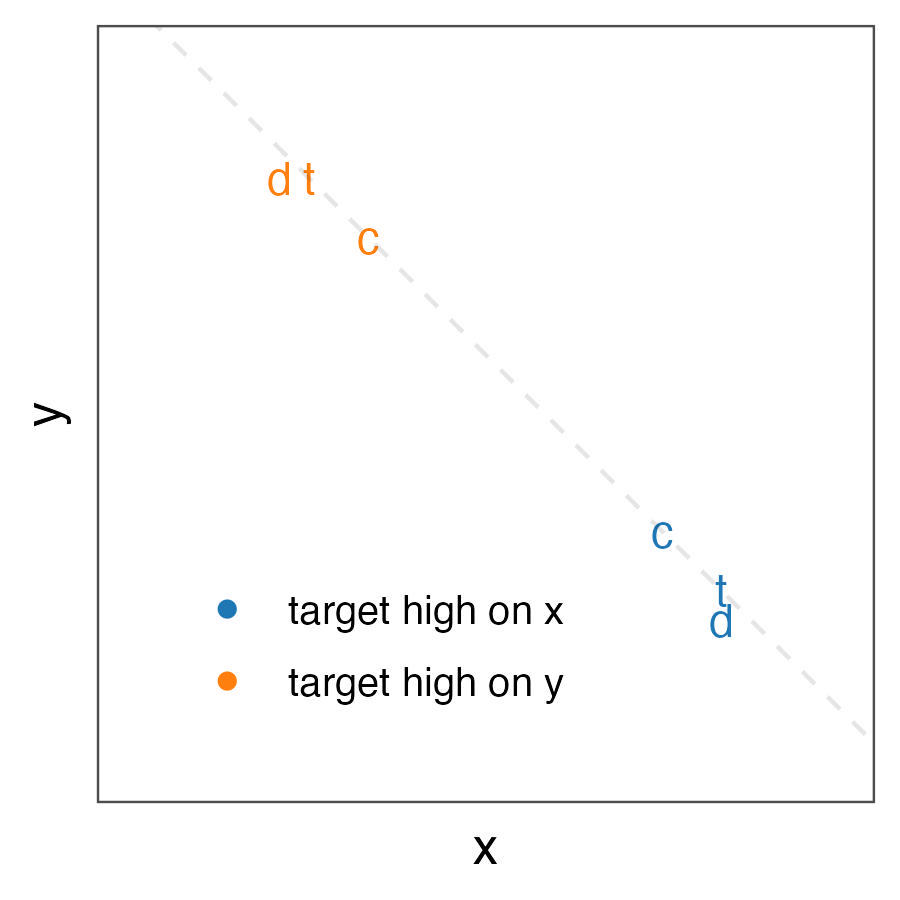
\includegraphics[width=150mm]{figures/banerjee_stim.jpeg}
    \caption{Graphical depiction of a subset of the stimuli used in \textcite{banerjeeFactorsThatPromote2024}, Experiment 5. Target, competitor, and decoy are labeled \textit{t}, \textit{c}, and \textit{d}, respectively. Dimensions are (generically) labeled X and Y. The choice sets vary based on whether the target is higher on the X or Y dimension. The dashed line is the diagonal line of indifference, assuming equal weighting of both the X and Y dimensions.}
    \label{fig:banerjee_stim}
\end{figure}

\textcite{banerjeeFactorsThatPromote2024}'s experiments compared binary to ternary choice rather than ternary to ternary choice, as in \textcite{spektorWhenGoodLooks2018b}. To do a ternary-ternary comparison, one would switch the target and competitor labels, such that the target is the intermediate option, the competitor is the extreme option, and the decoy is nearby the new, intermediate target. Though \textcite{banerjeeFactorsThatPromote2024} were able to generate violations of regularity in this binary-ternary comparison, the results are somewhat limited by the fact that the target was always more extreme than the competitor. In other words, though \textcite{banerjeeFactorsThatPromote2024} demonstrated that the choice share of the competitor option increased with the introduction of the decoy, this result may be due to extremeness aversion, decision-makers' tendency to not prefer options positioned more extremely in attribute space \parencite{simonson1992choice}. The introduction of the decoy may highlight the fact that the target is positioned particularly extremely compared to the target. For example, see their stimuli plotted in Figure~\ref{fig:banerjee_stim}. Consider the blue choice set, where the target is high on dimension $X$. Both $T$ and $C$ are relatively high on the $X$ dimension and low on the $Y$ dimension. $C$ is, however, higher on $Y$ while $T$ is higher on $X$. In choosing $T$ over $C$, consumers are forced to trade a small improvement in the $X$ dimension for an option with a particularly dismal $Y$ value. The introduction of the decoy may draw further attention to the $Y$ dimension, leading to greater choice for $C$ over $T$. This result is quite different than the results of \textcite{spektorWhenGoodLooks2018b}, because the decoy was never positioned near the less extreme option. 

\textcite{banerjeeFactorsThatPromote2024} argued that their results are consistent with the tainting hypothesis because the repulsion effect is strongest when the target and decoy are similar. The tainting hypothesis is the idea that the decoy can sometimes diminish the perceived value of the nearby target \parencite{frederick2008attraction}. They also argued that the decoy may have caused participants to focus more attention on the competitor's superior dimension. For example, in the blue choice set of Figure~\ref{fig:banerjee_stim}, the decoy is quite poor on $Y$ while being equally good as the target on $X$, so participants may have focused more attention on $Y$, leading to a preference for the competitor. 

\textcite{banerjeeFactorsThatPromote2024}'s results are worth exploring further. The current study uses their stimuli to measure participants' valuations of consumer products as well as collect choices from the same sets of products.

\section{Experiment 4}

The goal of Experiment 4 was to collect ratings and choice data in a preferential choice setting using (a subset of) \textcite{banerjeeFactorsThatPromote2024}'s Experiment 5 stimuli. These data were used to estimate the parameters of the choice model from Chapter 2. 

For a ratings measure, participants were told assign selling prices to each option. Though people often overestimate prices \parencite{breidertREVIEWMETHODSMEASURING2006}, pricing measures are approximately continuous\footnote{Here they only varied down to a single dollar. Thus, prices are approximately, but not perfectly, continuous.} and monotonic with value \parencite{miller2011should} and are thus comparable to estimated area, the value measure in Experiment 2.

\subsection{Methods}

\subsubsection{Participants}
137 U.S. adults participated in the experiment. Participants were recruited from Prolific, an online platform for research studies, and they were paid $\$5$ for their participation. 24 participants were removed from all analyses for failing catch trials (see below), leaving a final sample size of $N=113$. 
% The mean age was $38.89$ ($SD=11.48$). $61$ participants identified as female, $50$ identified as male, $1$ participant identified as non-binary, and $1$ participant preferred not to say.

\subsubsection{Stimuli}

The stimuli were borrowed from \textcite{banerjeeFactorsThatPromote2024}'s Experiment 1. The stimuli were hypothetical consumer choice products. All stimuli varied on two attributes, each of which ranged from 0-100. The products came from four different categories: televisions, washing machines, laptops, and microwave ovens. 

In each phase, there were two types of trials: critical trials and catch trials. The critical trial stimuli are shown in Figure~\ref{fig:ce_rating_stim}. 

There were two types of critical trials: those designed to elicit the repulsion effect (a replication of \citeauthor{banerjeeFactorsThatPromote2024}), and those designed to elicit the attraction effect (because the stimuli are located in the center of the attribute space with a decoy near one of two the focal options). These trials will be referred to as repulsion and attraction trials.

Within both the attraction and repulsion trials, the stimuli varied on which dimension the target was higher on (1 or 2), $TDD$ (designated near or far from the target), and product category (microwaves, washing machines, laptops, and televisions). Note that to create the attraction trials, the target and competitor were shifted towards the center of the attribute space. That is, target and competitor are equally similar in both repulsion and attraction trials, but they are both more extreme in the repulsion trials.

\begin{figure}
    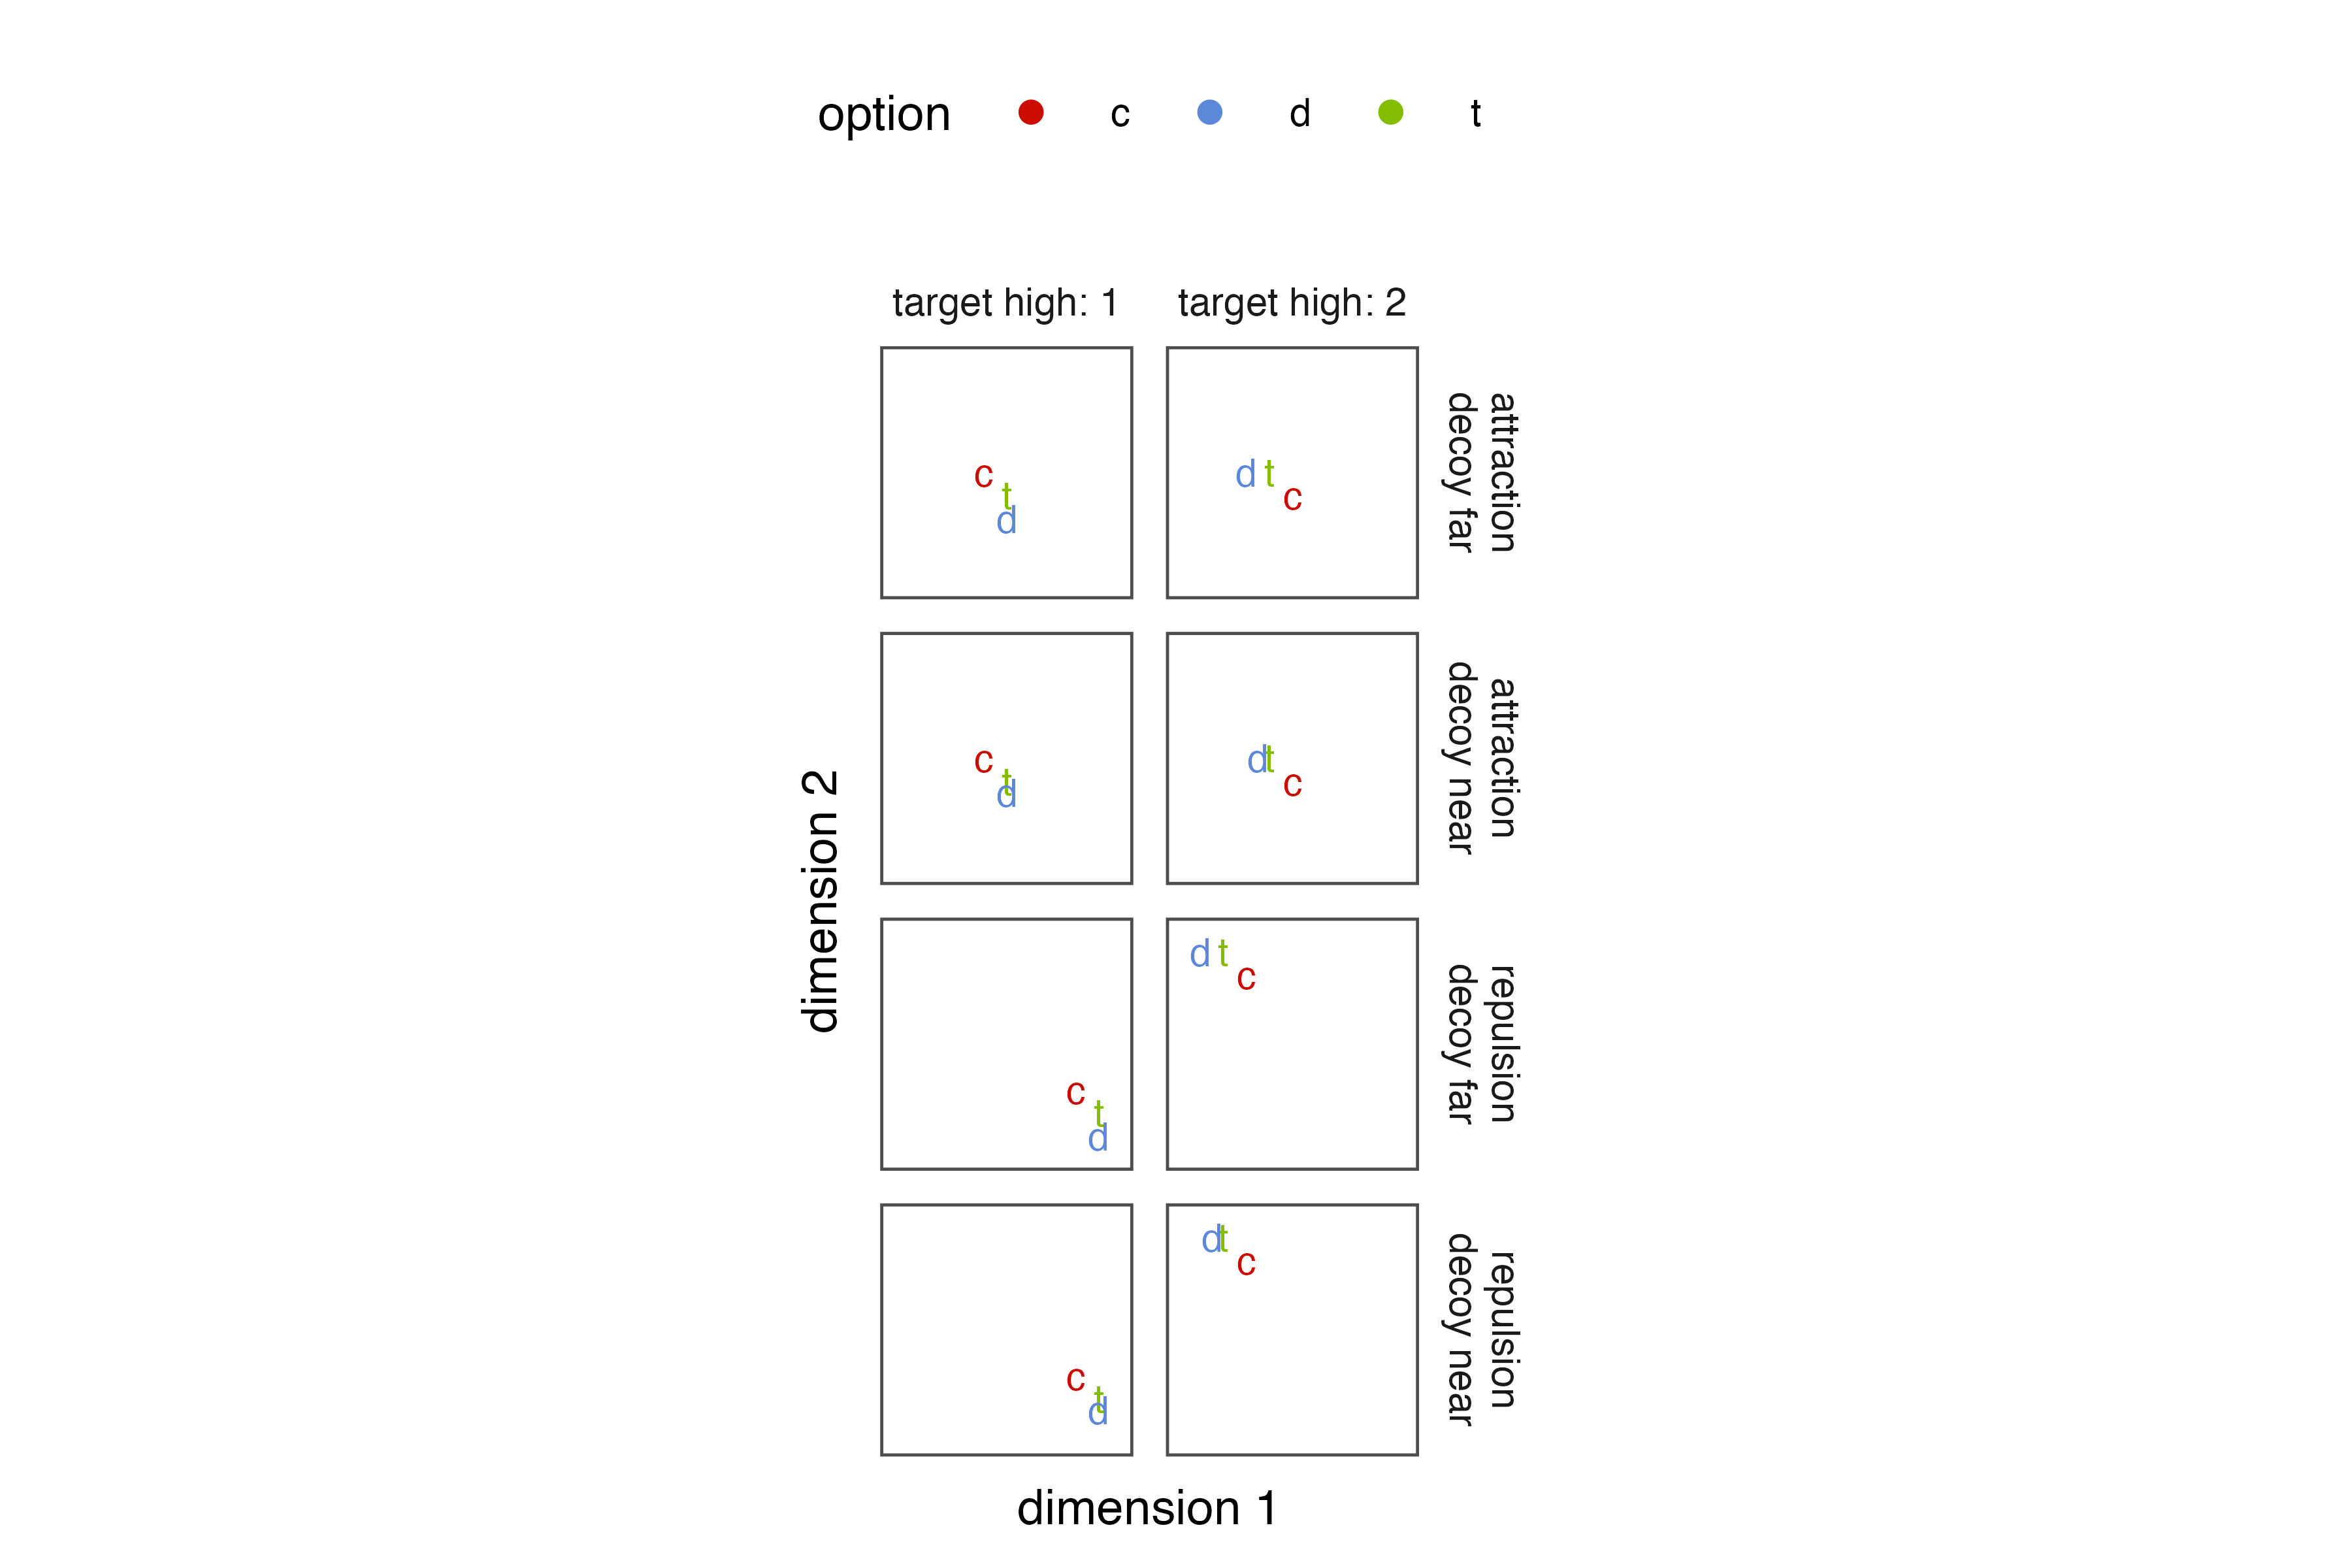
\includegraphics[width=150mm,scale=0.5]{figures/ce_rating_stim_for_paper.jpeg}
    \caption{Graphical depiction of the critical stimuli from Experiment 4. Rows show the different choice sets designed to elicit the attraction/repulsion effect, with the label also specifying whether the decoy is near or far from the target in attribute space. The columns indicate which dimension the target is high on (1 or 2). Dimensions are labelled generically because their names vary with product category.}
    \label{fig:ce_rating_stim}
\end{figure}

The attribute names varied by category. Televisions varied on screen size and average lifespan. Washing machines varied on average lifespan and energy savings. Laptops varied on processing speed and memory (RAM). Microwave ovens varied on warranty and cooking power. 

Within each category, one attribute was arbitrarily designated as dimension 1 and another as dimension 2. However, the order of attributes was randomized on each trial.

The catch trials were designed such that one option was clearly superior to the other two. On each catch trial, the superior option's dimension values were each independently sampled from the vector $[50,55,60,65,70,75,80,85,90,95]$, while the two inferior options' dimension values were independently sampled from the vector $[5,10,15,20,25,30,35,40,45,50]$. 

\subsubsection{Design}

The experiment took place in two phases: pricing and choice. The stimuli were identical for both phases.

As discussed above, there were both critical trials and catch trials in each phase. 

In both the rating phase and the choice phase, there were 32 critical trials - 16 designed to elicit the repulsion effect and 16 designed to elicit the attraction effect - along with 8 catch trials.

The experiment did not contain binary repulsion effect trials, as in \textcite{banerjeeFactorsThatPromote2024}'s experiments, so this chapter cannot assess the repulsion effect to the same degree as those authors. The goal of this experiment was to measure valuation correlations in consumer preference and relate them to choice.

\subsubsection{Procedure}

The experiment took place in two phases: a pricing phase and a choice phase.

Prior to the pricing phase, participants were provided with a cover story. According to the cover story, they were told to imagine that they run an online consumer goods resale business. On each trial, they would see three products, and they needed to determine which price to sell each product for. Participants were told that the ratings varied from 0 to 100, where 0 was the lowest possible rating and 100 was the highest possible rating. Participants were also told that they should determine a price that maximizes both profit and the likelihood the product is purchased. 

During the pricing trials, the three options were presented in a table, with the options in rows and the attributes in columns. All attributes were represented numerically. The options were labeled A, B, and C. The last column of the table contained three boxes, which participants used to type in their selling price for each option. Participants typed in their selling price and then clicked a button on the screen to advance to the next trial. Both option order and dimension order was randomized on each trial. See Figure~\ref{fig:ce_rating_choice_trial} (left panel) for an example trial. Participants were only allowed to enter in whole numbers (i.e., dollars not cents).

\begin{figure}
    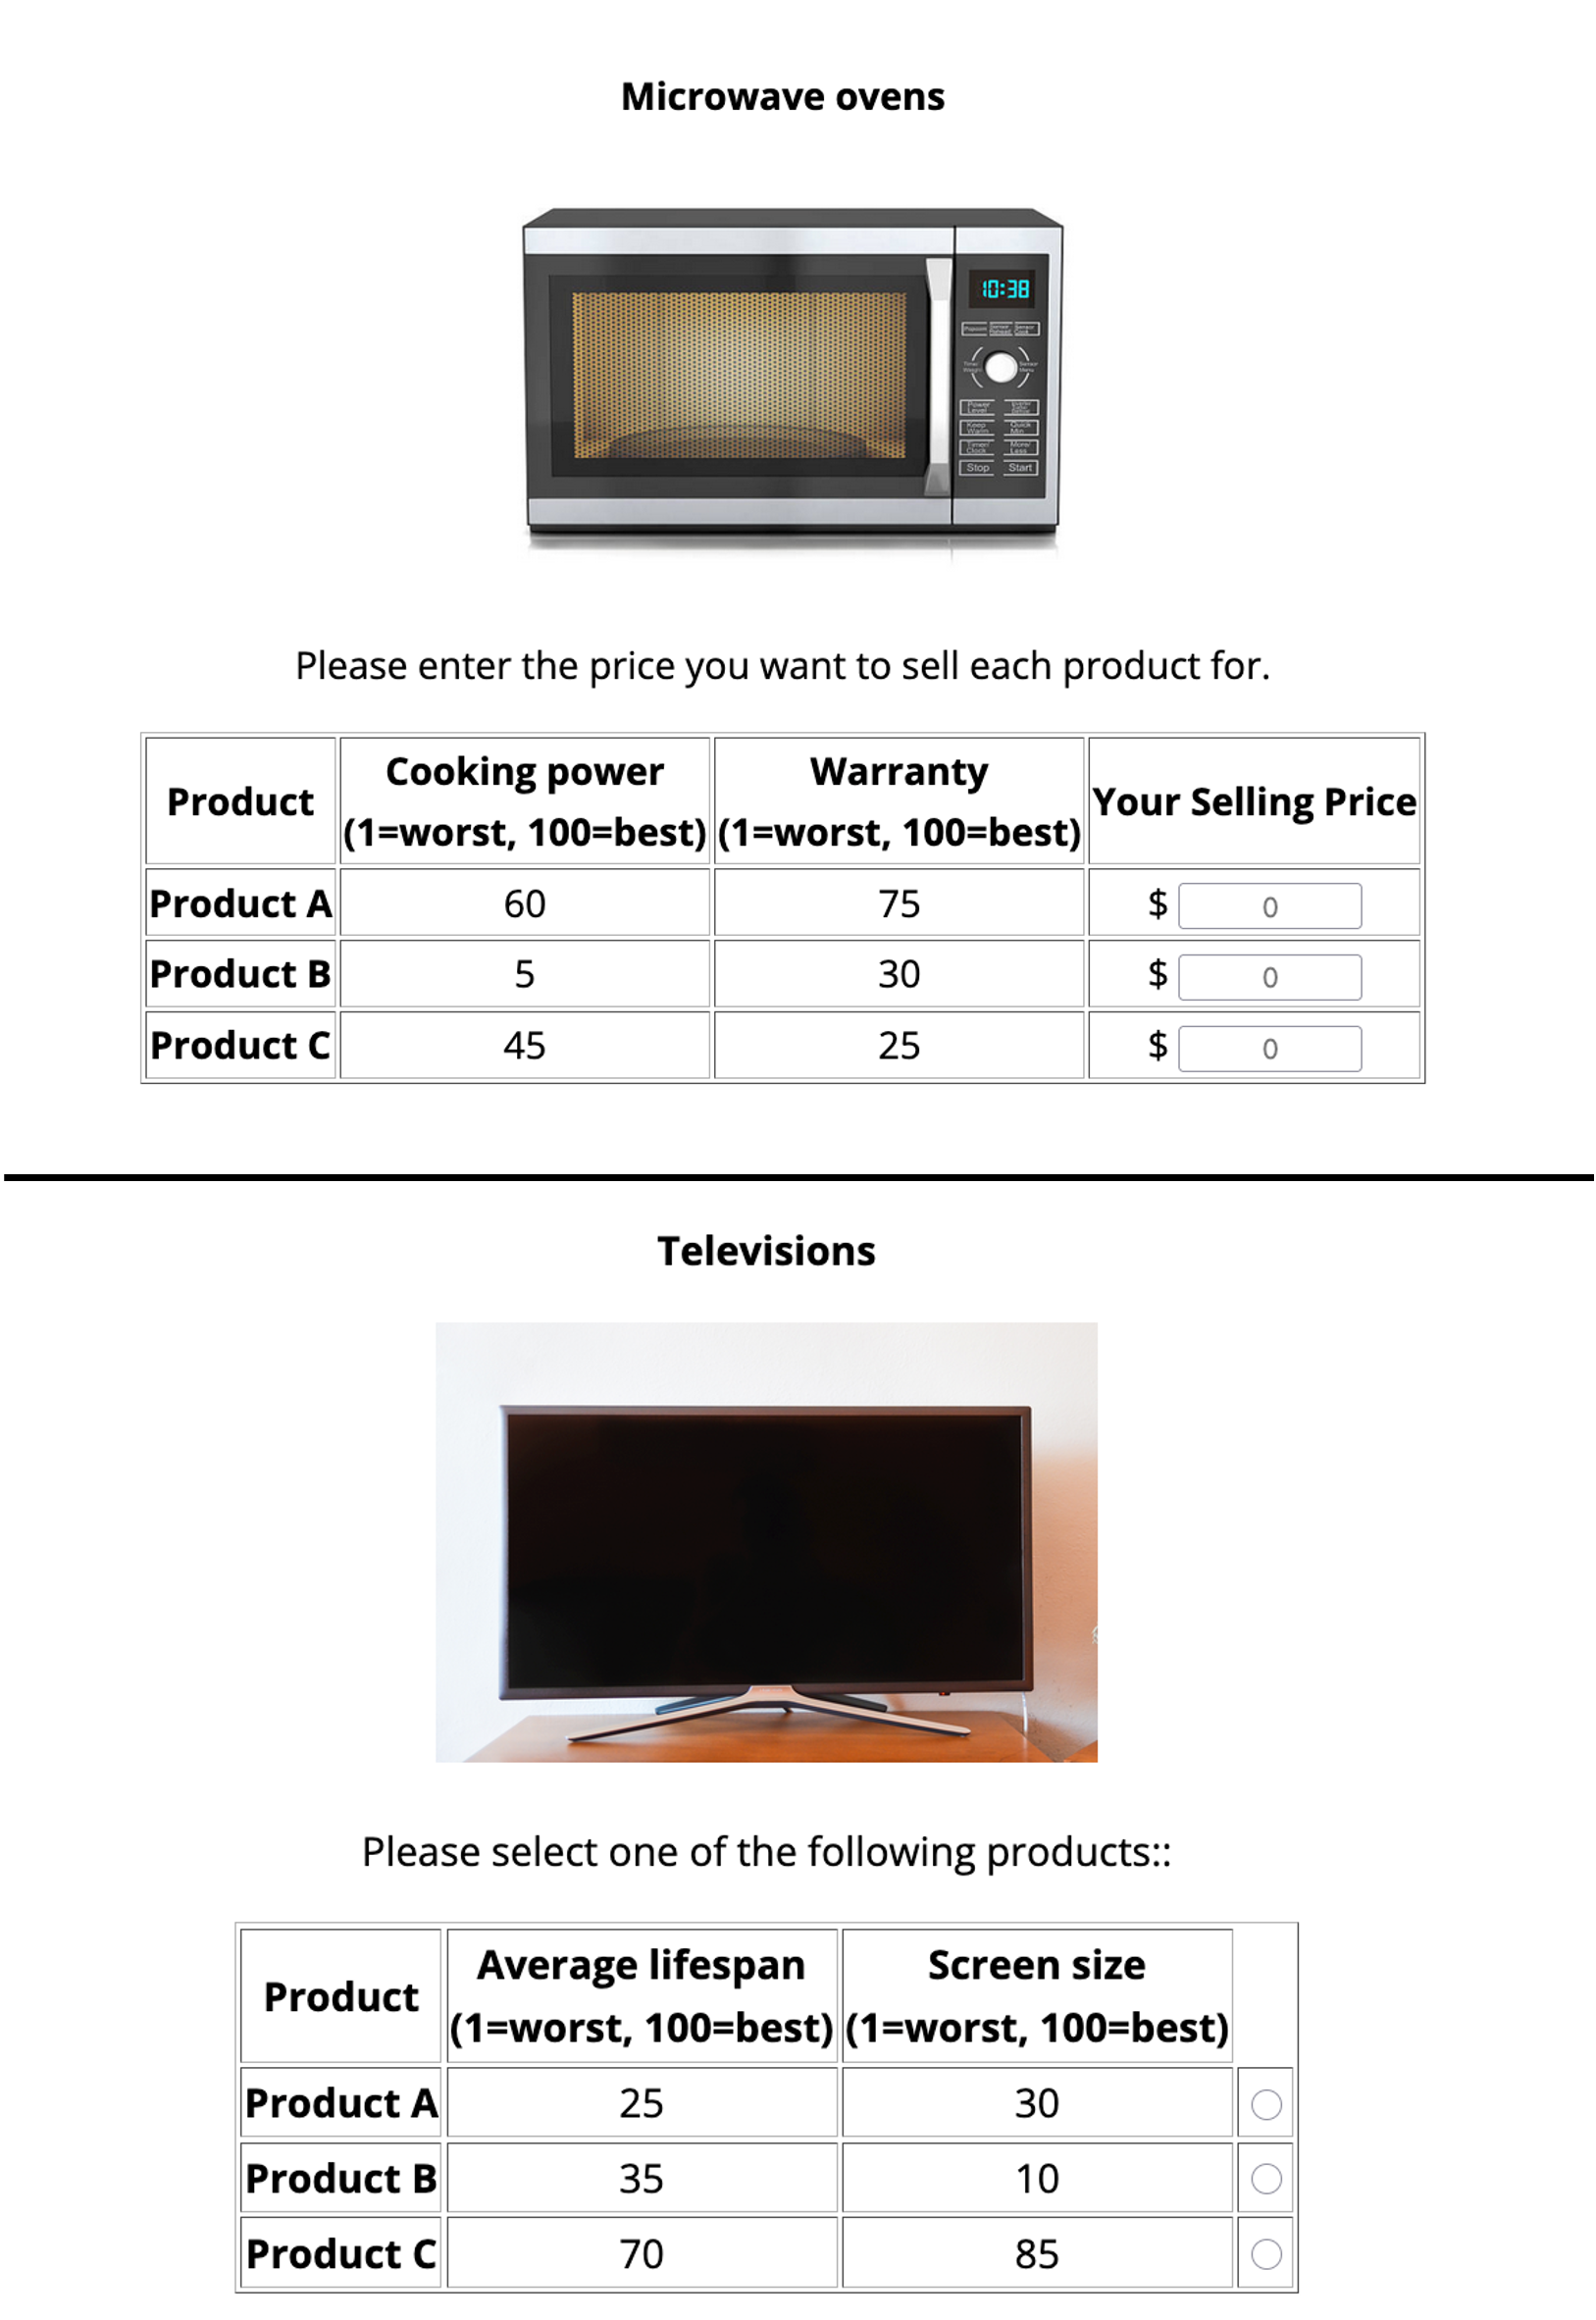
\includegraphics{figures/ce_rating_choice_example_trial.jpg}
    \caption{Sample trials from the pricing phase (top) and choice phase (bottom) in Experiment 4.}
    \label{fig:ce_rating_choice_trial}
\end{figure}

After completing all pricing trials, participants moved onto the choice phase. Prior to the choice phase participants were told to imagine that they were purchasing consumer goods in bulk. On each trial, they were to select the option they wanted to purchase. 

As in the pricing phase, options were presented in a table. See Figure~\ref{fig:ce_rating_choice_trial} (bottom) for an example trial.

In both phases, trial order and option order within each trial were randomized. 

After the choice phase, participants completed a short demographics form before the experiment ended. 

\subsection{Results}

\subsubsection{Data Processing}

First, 24 participants were removed from the data because they did not pass at least $5/8$ catch trials in both the pricing phase and the choice phase. To pass a pricing catch trial, the participant needed to price the superior option at least as high as the other two inferior options. To pass a choice catch trial, the participant needed to select the superior option. 

\subsubsection{Pricing Trials}

First, mean prices were computed for the target, competitor, and decoy options within each trial type and product category. These means are shown in Figure~\ref{fig:price_m_by_effect_category}.

On average, participants priced the target and competitor higher than the decoy. They also assigned higher prices to products that are typically more expensive (e.g., washing machines are more expensive than microwave ovens). This suggests that participants were engaged with the task and, in a relative sense, performed the task well.

\begin{figure}
    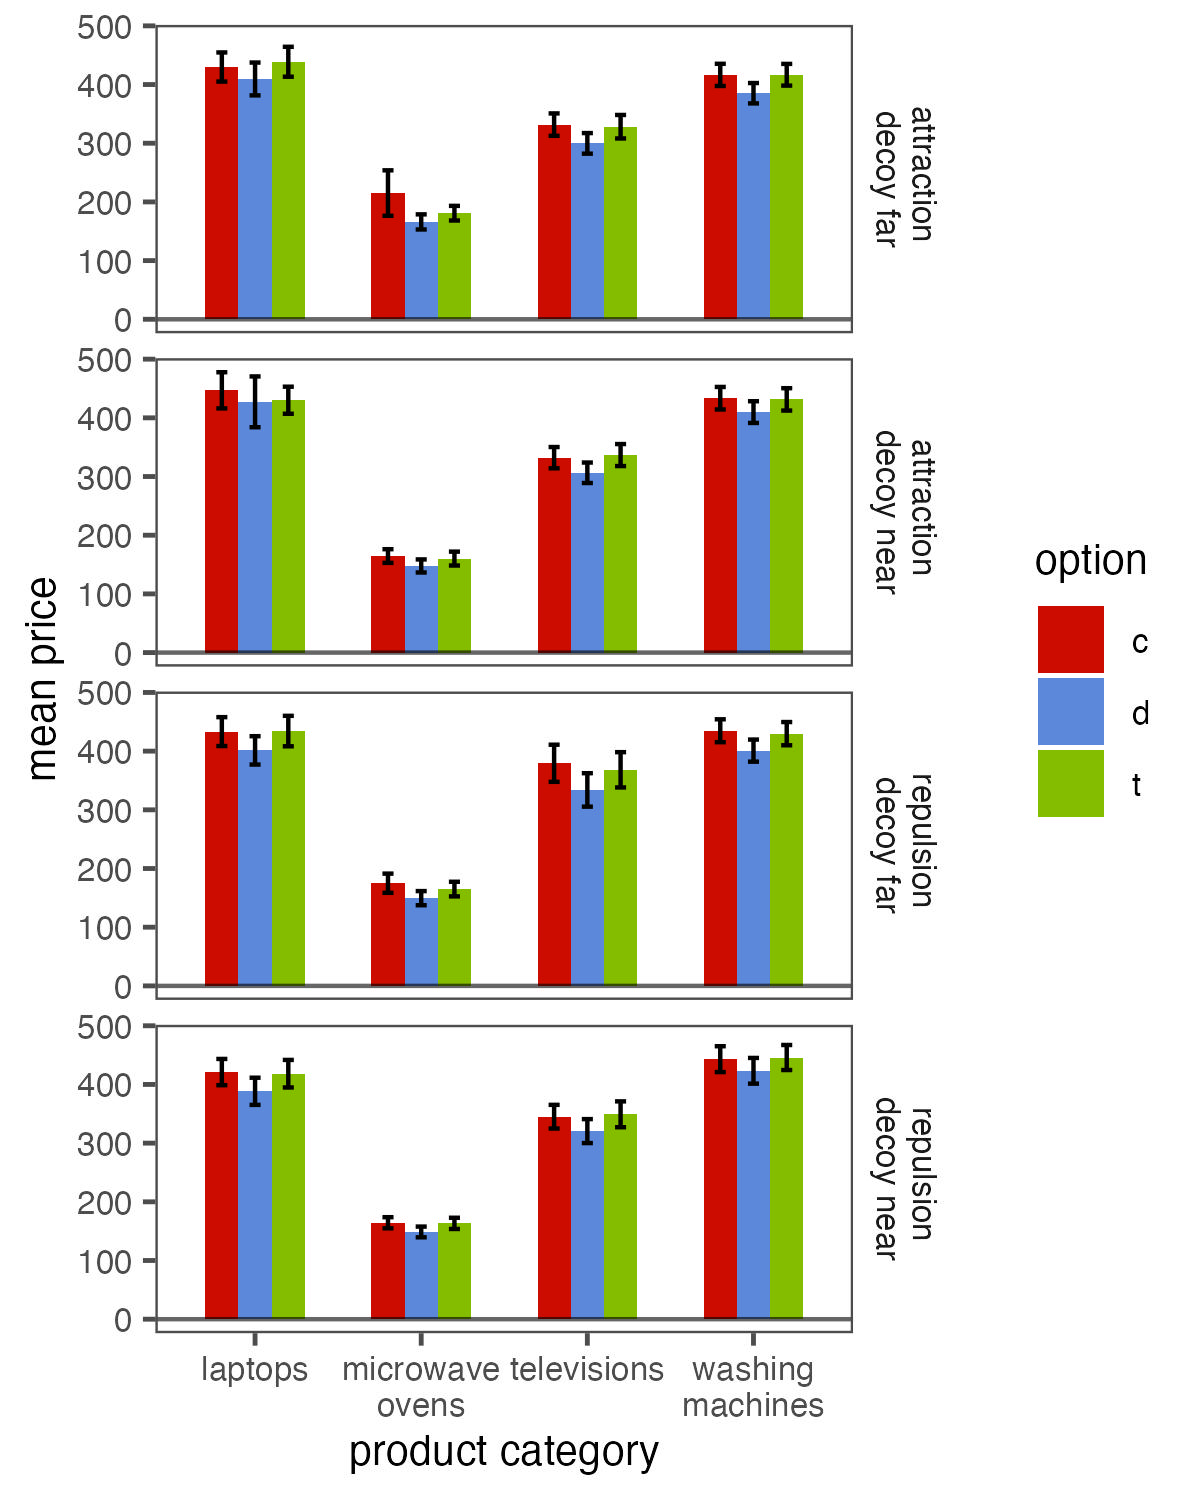
\includegraphics[width=130mm,scale=0.5]{figures/price_m_by_effect_category.jpeg}
    \caption{Experiment 4 mean prices by product category, option, and trial type. Error bars are $\pm 1\;\text{SEM}$.}
    \label{fig:price_m_by_effect_category}
\end{figure}

A Bayesian modeling analysis was performed to estimate the parameters of the Thurstonian choice model, comparable to that of Experiment 2. This analysis was used to estimate the means, variances, and correlations for the pricing data and perform inference on these data. The details of the estimation and the results are presented in the Apppendix, with the exceptions of the posterior distributions for several crucial parameters (i.e., means and correlations). The main text discusses descriptive statistics for these parameters, but whenever it is claimed that one parameter value is greater than another, the reader can see the Appendix for statistical inference which supports these conclusions. 
% The descriptive values for all correlations, rather than those based on model estimates, because the latter are  biased downard due to limited data \parencite{stephens2020state,merkle2023opaque}. 

To account for participant-level differences in pricing, all prices were normalized within each participant. To avoid the influence of outliers on correlation estimates, $33$ trials in which at least one price z-score had an absolute value $>3$ were also removed, leaving $3,583$ trials remaining. 

The mean prices were computed for target, competitor, and decoy options within each trial type, collapsing over product category and TDD, shown in Figure~\ref{fig:price_mu_model_data}. In both repulsion and attraction effect trials, the target and competitor did not differ in mean price, while both are priced higher than the decoy option.

\begin{figure}
    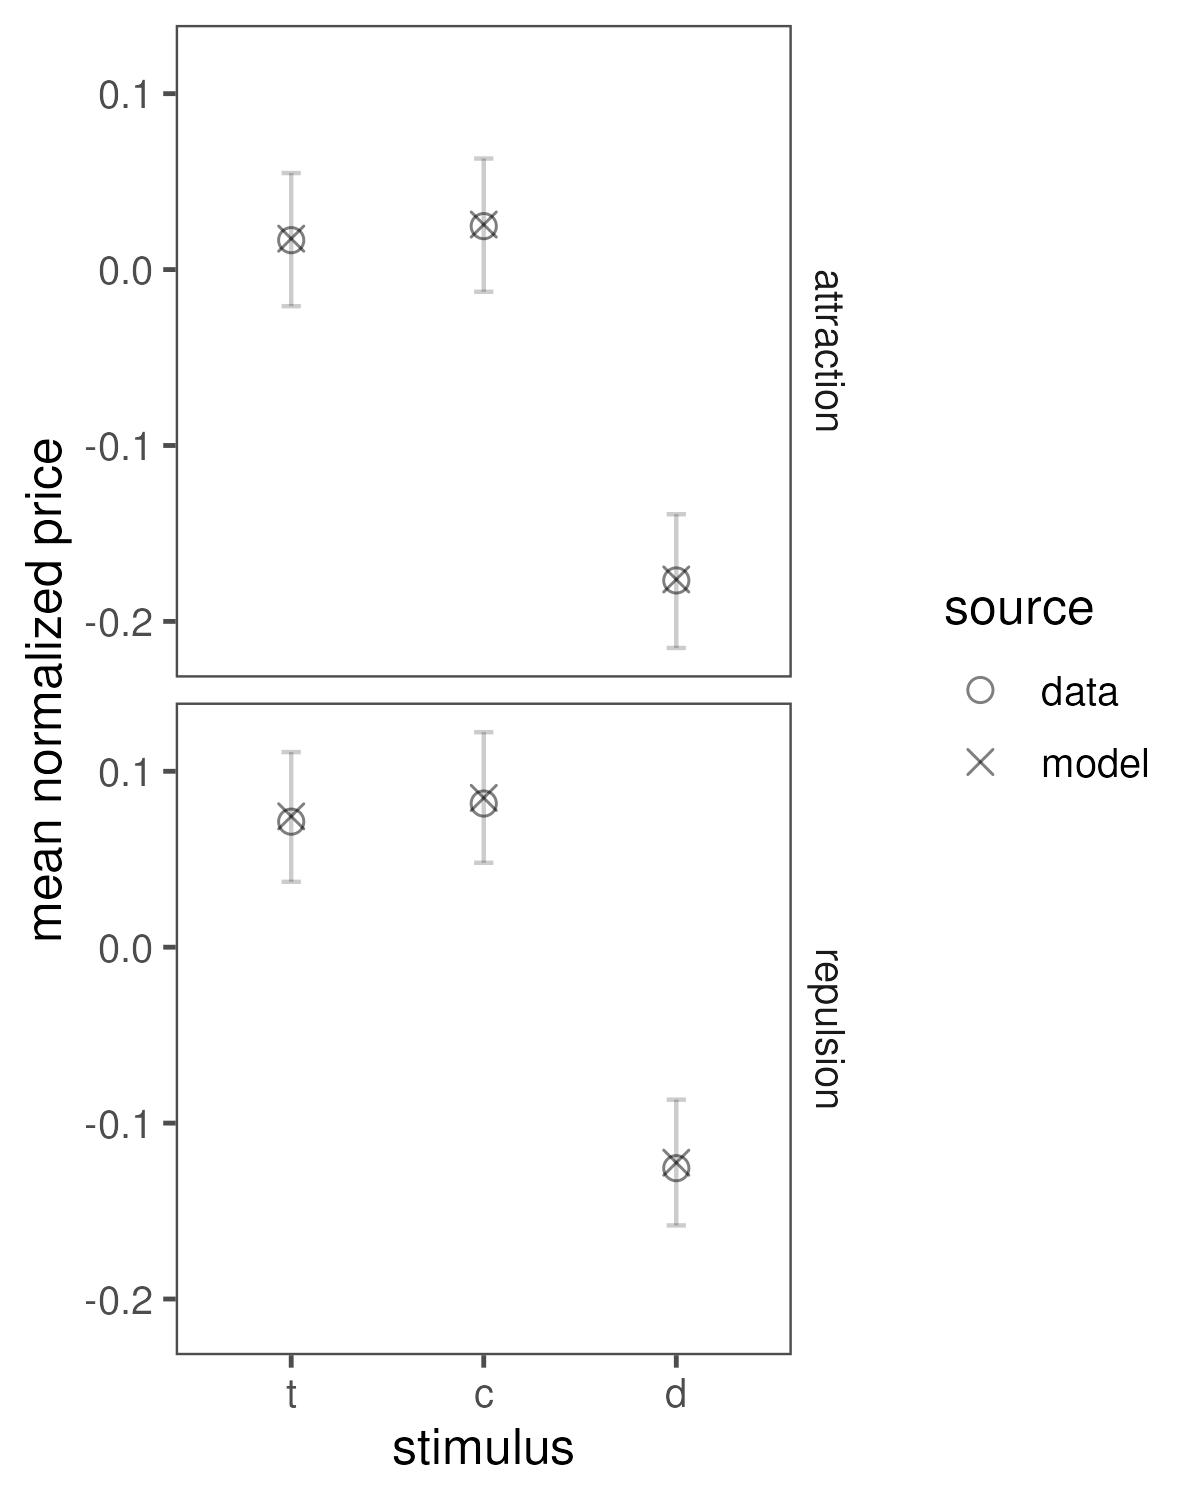
\includegraphics[scale=0.5, width=100mm]{figures/pricing_mu_model_data.jpeg}
    \caption{Experiment 4 mean prices for target, competitor, and decoy options in both repulsion and attraction trials. Model values are the means from the posterior distribution, and error bars are $95\%$ HDIs.}
    \label{fig:price_mu_model_data}
\end{figure}

Correlations between the prices assigned to options were computed within each trial type. The normalized prices are plotted in a series of scatterplots, with the Pearson correlations included. See Figure~\ref{fig:price_z_corplot_attraction} for attraction effect scatterplots and Figure~\ref{fig:price_z_corplot_repulsion} for repulsion effect scatterplots.

Note that in both Figure~\ref{fig:price_z_corplot_attraction} and Figure~\ref{fig:price_z_corplot_repulsion}, the decoy is occasionally priced hgiher than the target (i.e., the points above the diagonals in the target-decoy scatterplots). This may be due to participant inattention or response error, as the decoy should never be priced higher than the target provided adequate attention. 

\begin{figure}
    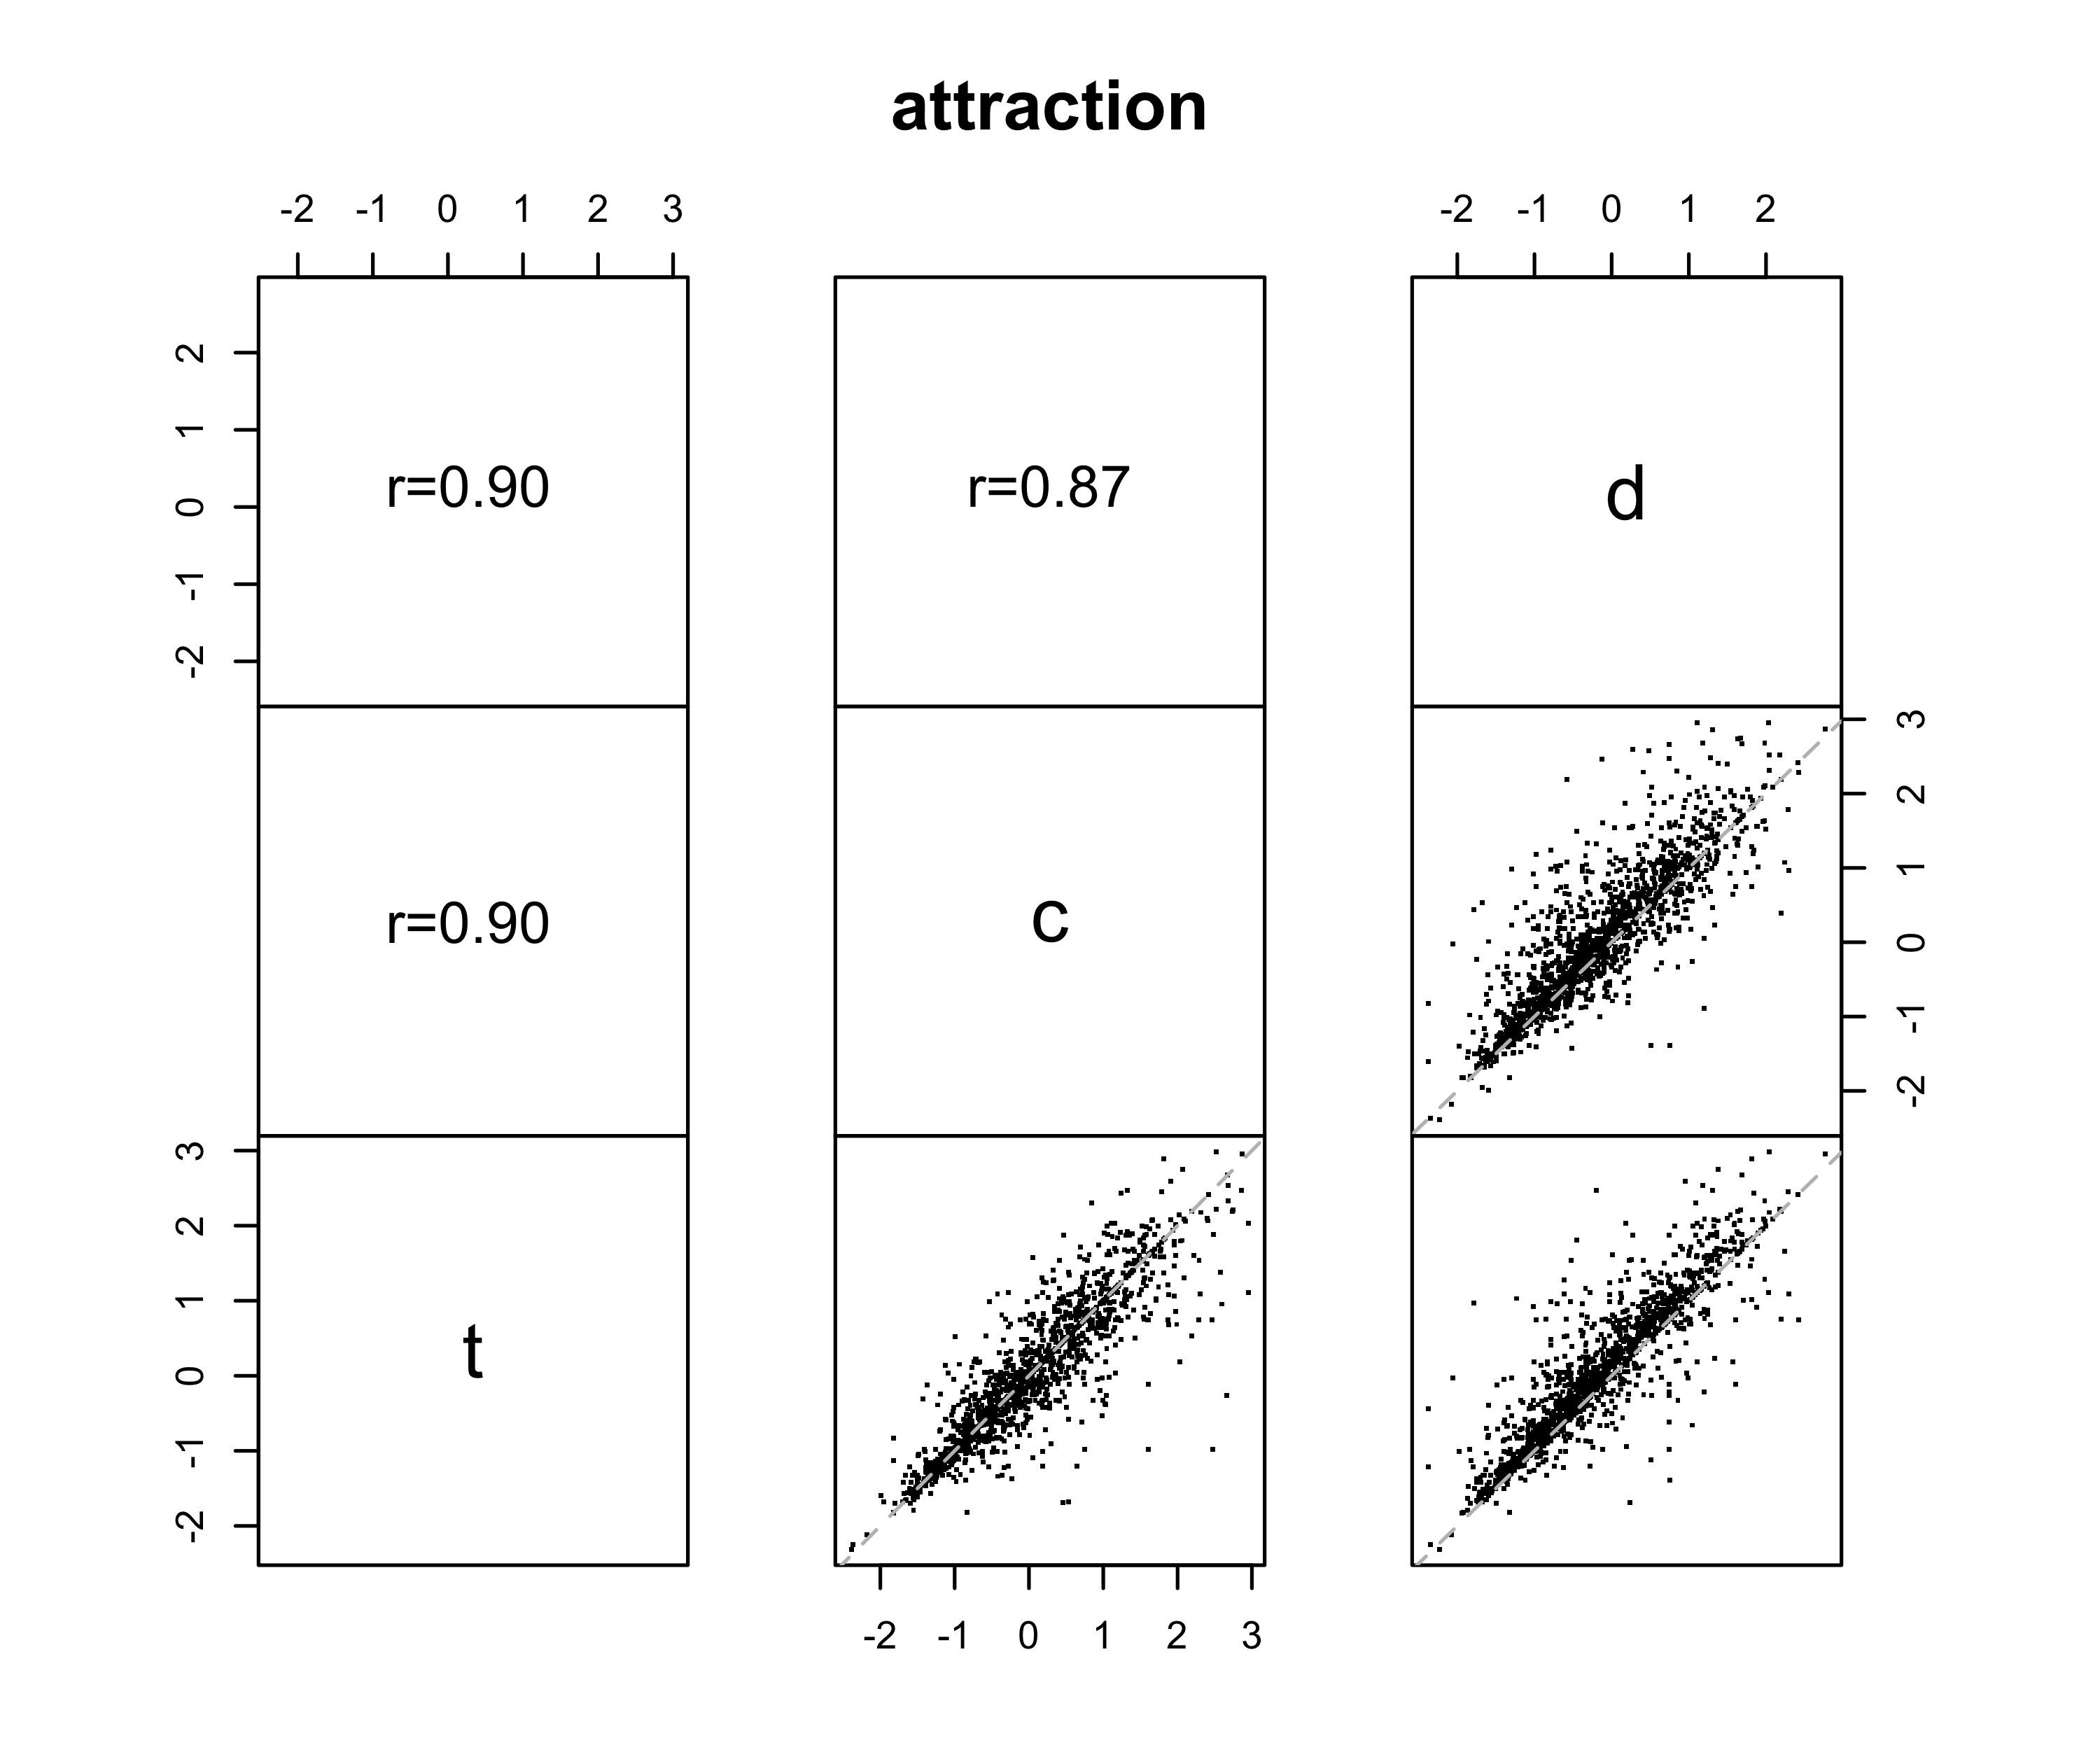
\includegraphics[scale=.5,width=120mm]{figures/price_z_corplot_attraction.jpeg}
    \caption{Experiment 4 correlation plots for all pairs of stimuli, in trials designed to elicit the attraction effect. t=target, c=competitor, and d=decoy.}
    \label{fig:price_z_corplot_attraction}
\end{figure}

\begin{figure}
    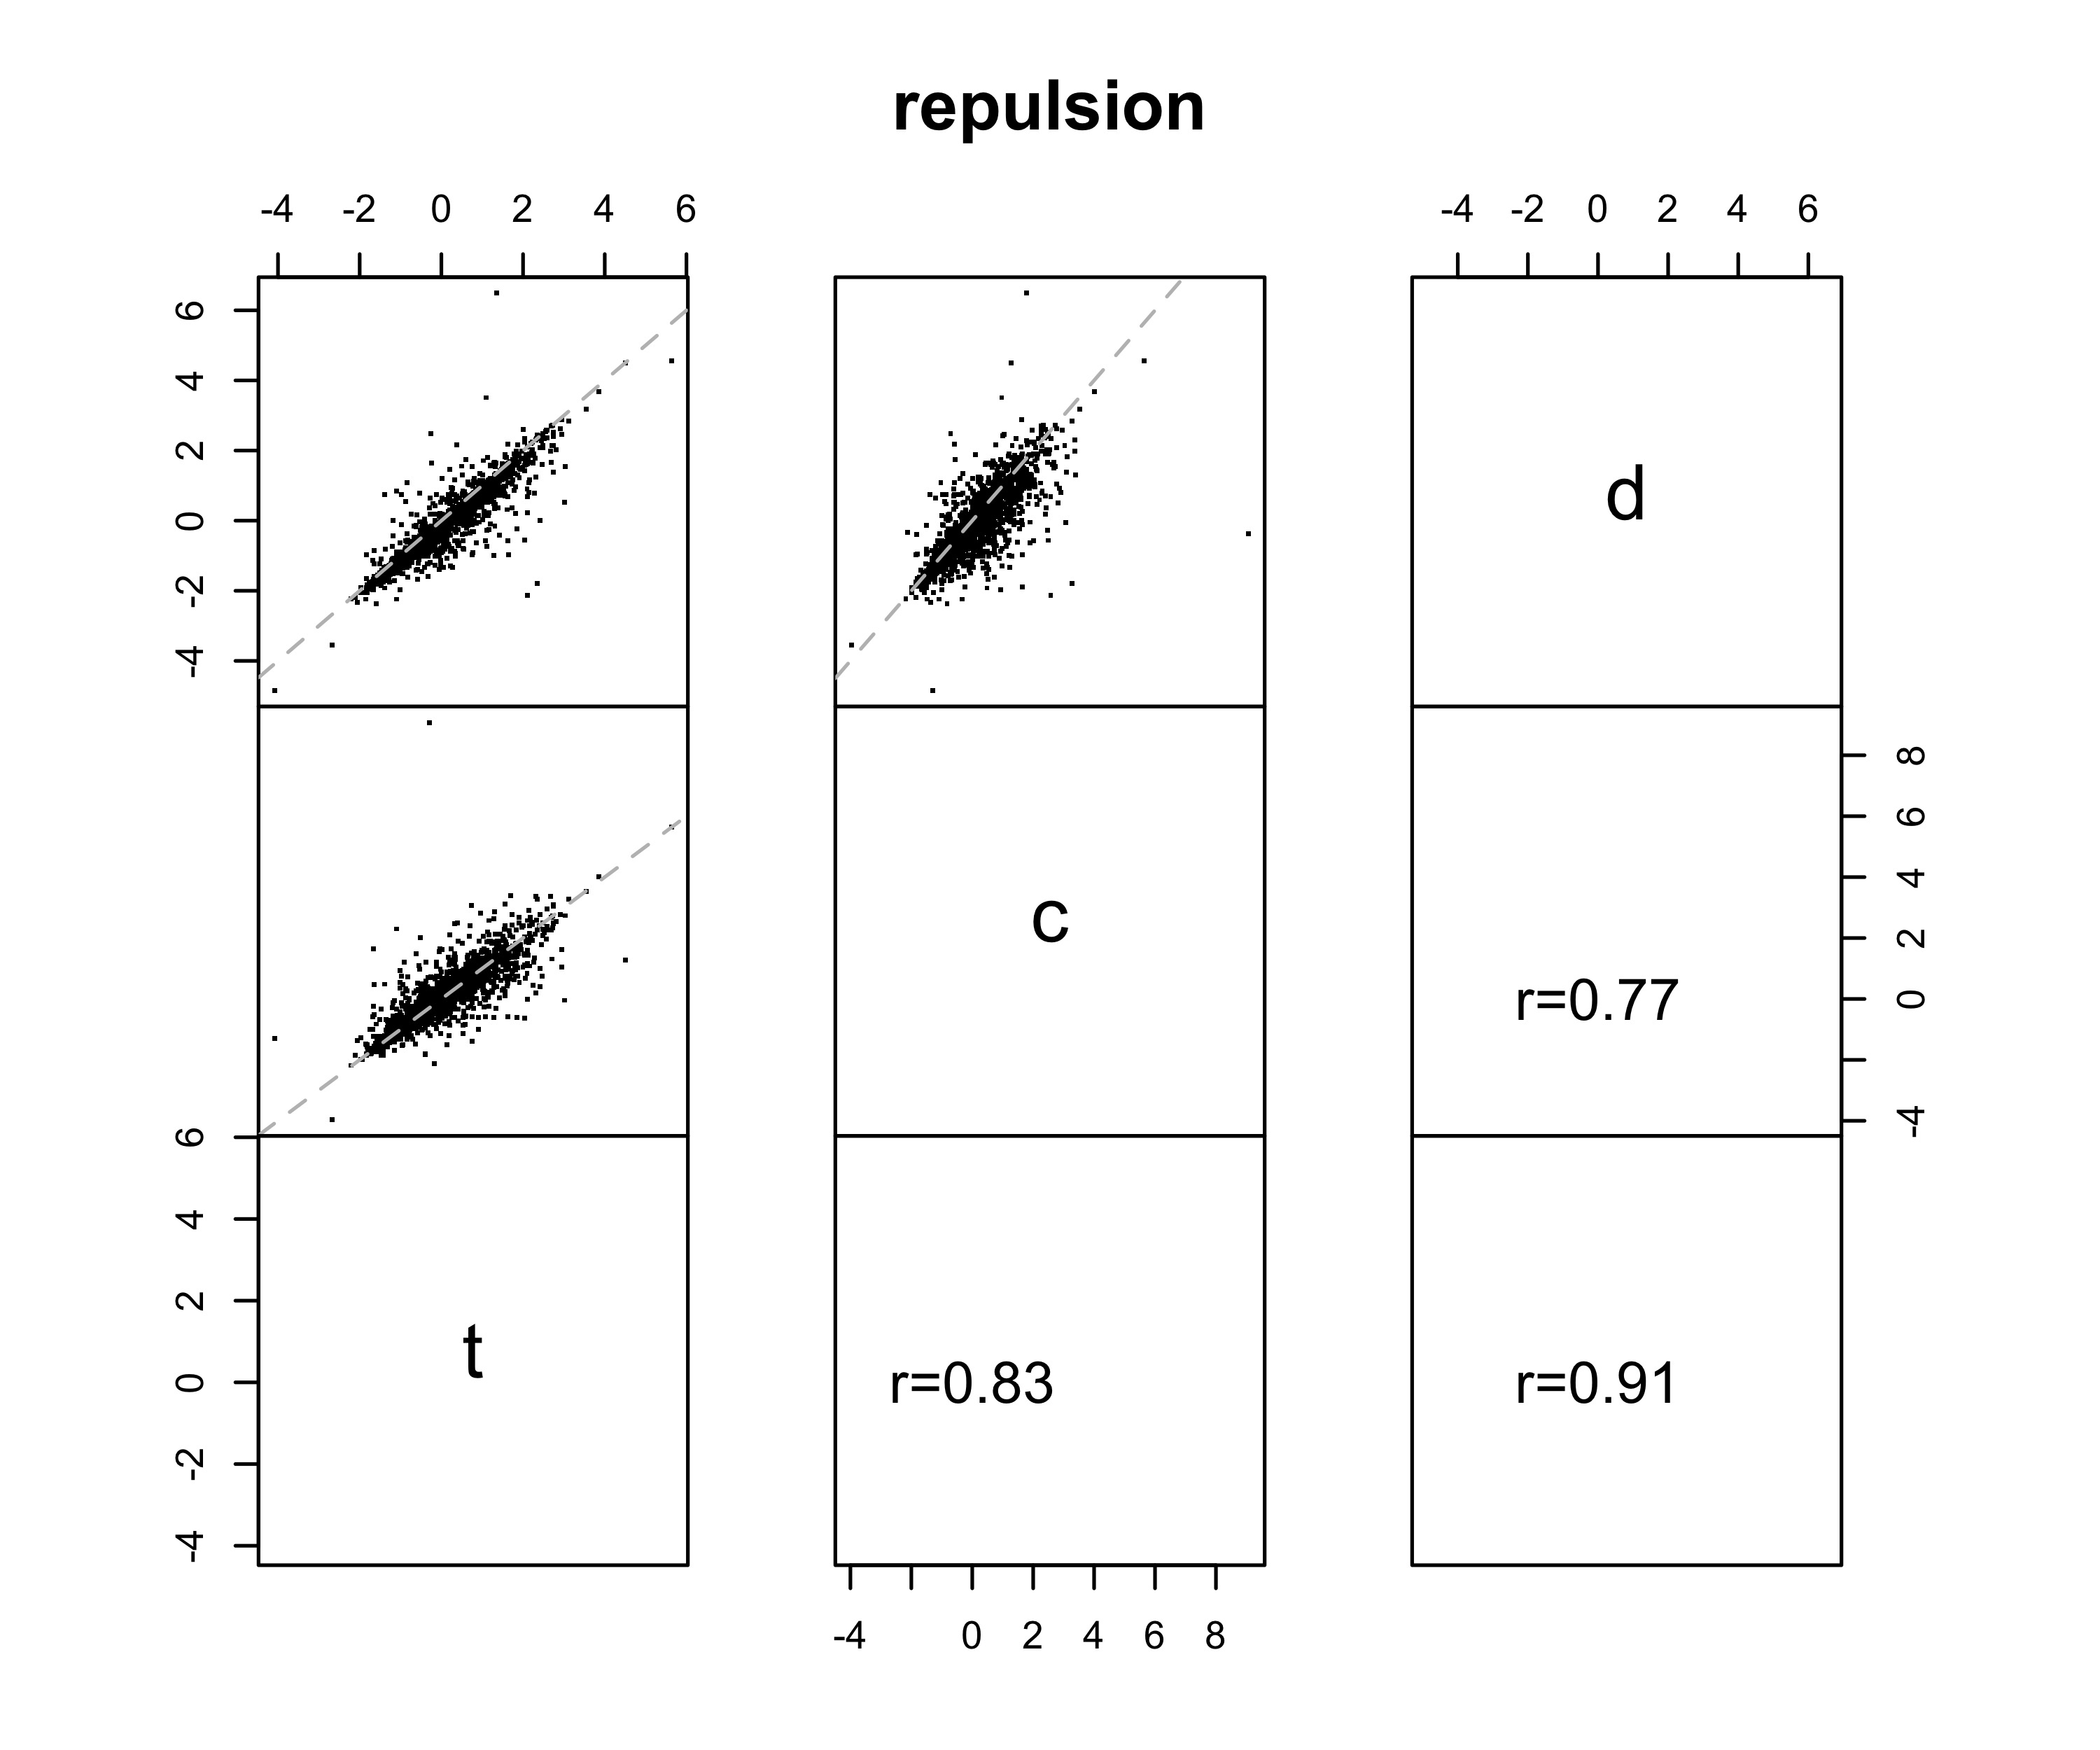
\includegraphics[scale=.5,width=120mm]{figures/price_z_corplot_repulsion.jpeg}
    \caption{Experiment 4 correlation plots for all pairs of stimuli, in trials designed to elicit the repulsion effect. t=target, c=competitor, and d=decoy.}
    \label{fig:price_z_corplot_repulsion}
\end{figure}

Posterior distributions of the correlation parameters are plotted in Figure~\ref{fig:price_omega}. The repulsion trials, replicated the results of Experiment 2, in that $\rho_{TD}>\rho_{TC}$ and $\rho_{TD}>\rho_{CD}$. The results also showed that $\rho_{TC}>\rho_{CD}$, while in Experiment 2 $\rho_{TC}\approx\rho_{CD}$. In the attraction trials, the correlations showed a slightly different pattern, where $\rho_{TC}\approx\rho_{TD}>\rho_{CD}$. In other words, the target and competitor are approximately equally similar as target and decoy, which are in turn more similar than competitor and decoy. 

\begin{figure}
    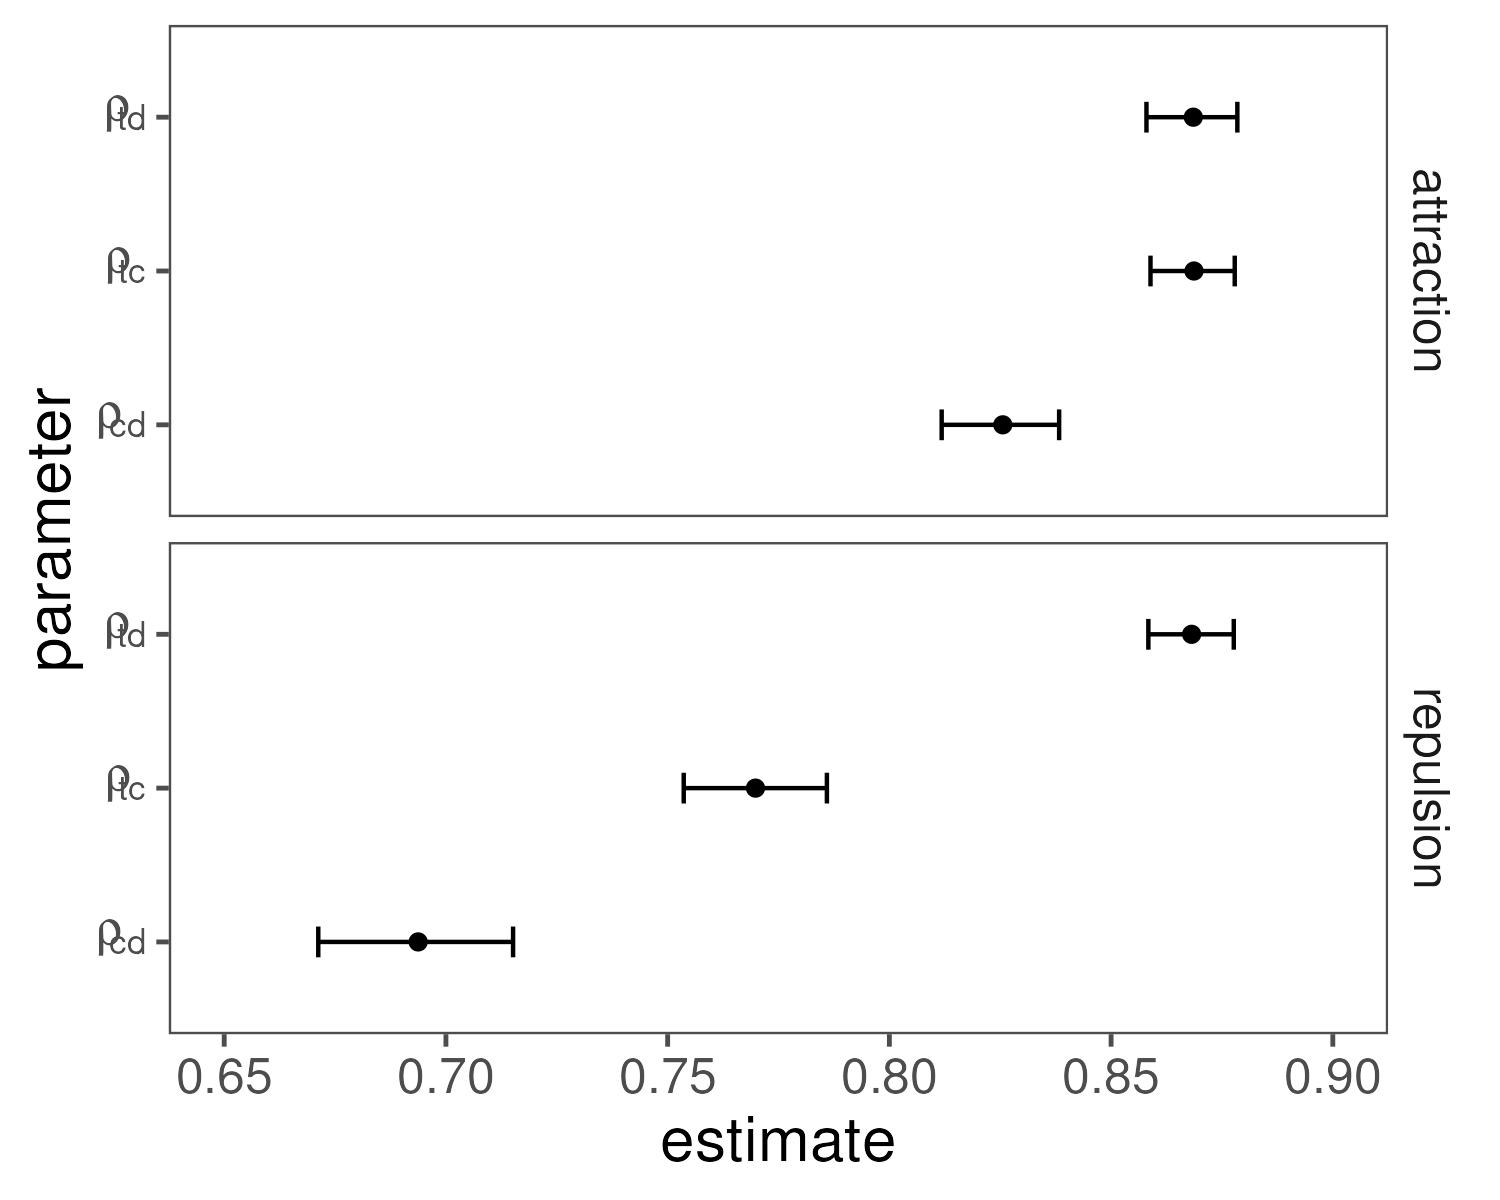
\includegraphics[scale=.5,width=120mm]{figures/price_omega_posteriors.jpeg}
    \caption{Experiment 4 posterior distributions on correlation parameters. Dots are means, and error bars are $95\%$ HDIs.}
    \label{fig:price_omega}
\end{figure}

\subsubsection{Choice Trials}

Next, the choice proportions were computed for the critical choice trials. These results are collapsed across participant (due to the small $n$ per subject), product category, and the target's superior dimension.

Participants seldom chose the decoy, an indication that they were attentive to the task. This also provides evidence that decoy selection is far more common in perceptual choice than preferential choice.

These aggregate choice proportions are plotted in Figure~\ref{fig:bayes_choice_model_data_plot}. The results clearly show a null attraction effect, regardless of $TDD$. Participants chose the target and competitor options at equal rates. This is likely due to the strong similarity of target and competitor. The target and competitor were particularly close to one another, a design which is atypical of attraction effect studies. 

The results show a strong repulsion effect, where the participants generally prefer the competitor option to the target option. These data replicate the results of \textcite{banerjeeFactorsThatPromote2024}, albeit without the binary-ternary comparison included in their experiments. These results may be due to participants simply preferring the less extreme option, as discussed in the introduction to this chapter.

See the Appendix for statistical inference which supports these conclusions.

\begin{figure}
    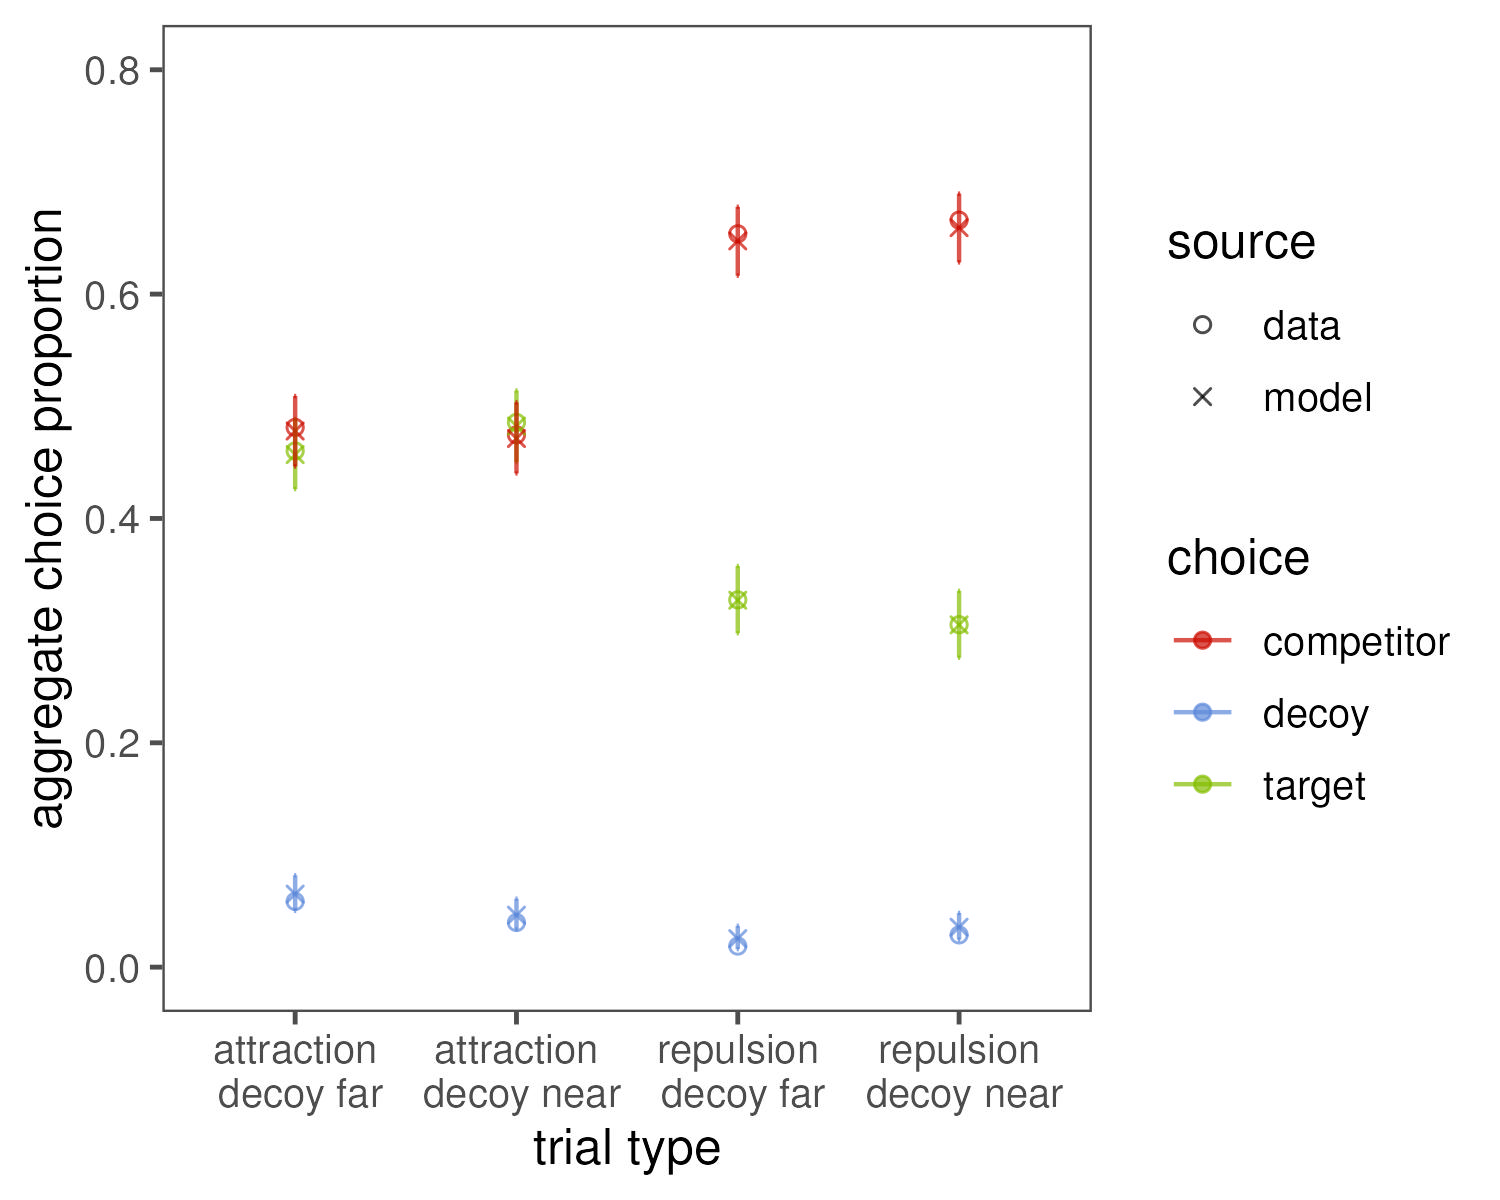
\includegraphics[scale=.5,width=100mm]{figures/bayes_choice_model_data_plot.jpeg}
    \caption{Experiment 4 aggregate choice proportions for each trial type, TDD, and option. Data points are aggregate choice proportions, while model points are posterior means computed from the Bayesian Dirichlet-multinomial model presented in the Appendix. Error bars are $95\%$ HDIs.}
    \label{fig:bayes_choice_model_data_plot}
\end{figure}

\subsubsection{Model Simulations}

As in Chapter 2, the Thurstonian choice model conditional on the parameter estimates,i.e., $\boldsymbol{\mu}$ and $\boldsymbol{\Sigma}$, were used to simulate choice. Though the model was originally applied to perceptual choice, it is a general purpose choice model where the primary dimension is value, and the model is agnostic about what this value refers to. 

As in Chapter 2, the model assumes that value is stochastic while choice is deterministic\footnote{This assumption also assumes ties are not possible, which is true if and only if value is truly continuous.}. The model always chooses the option perceived as most valuable, regardless of the magnitude of the difference between the winner" and runners-up. That is, given a vector $\mathbf{X}_i$ of perceived values on trial $i$ with set $K$, the probability a participant selects stimulus $j$ is:

\begin{align}
   P(j|i,K)=P(\mathbf{X}_{ij}>\mathbf{X}_{ik}), \forall k \in K, j \neq k
   \label{eqn:pchoice_price}
\end{align}

$1,000,000$ simulations of the model were run, with the results plotted against the data in Figure~\ref{fig:bayes_choice_sim_preds}.

\begin{figure}
    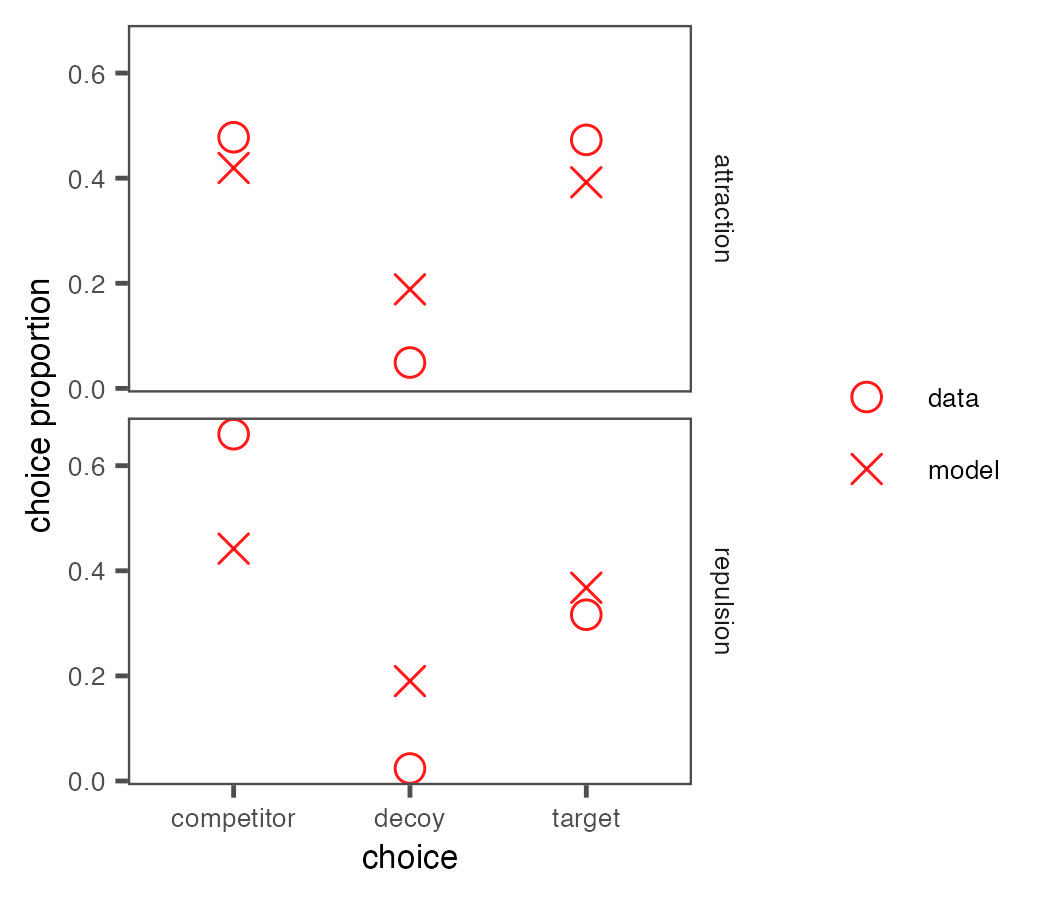
\includegraphics[scale=.5,width=100mm]{figures/bayes_choice_sim_preds.jpeg}
    \caption{Experiment 4 data vs. Thurstonian model predictions.}
    \label{fig:bayes_choice_sim_preds}
\end{figure}

The model mispredicts the attraction trials. It predicts a slight repulsion effect when in fact the data suggest a null effect. This is similar to the results of Experiment 2 (horizontal condition), where the model predicted a repulsion effect even when the empirical data showed a repulsion effect, due to the influence of the target-decoy correlation.

The model does, however, successfully predict a qualitative repulsion effect, i.e., $P(C)>P(T)$. However, it strongly overpredicts the decoy choice proportions. It also underpredicts competitor choice proportions. The model relies on the correlation between target and decoy choice proportions to predict the repulsion effect. According to the model because the target and decoy are strongly correlated, it is more likely that the utility of the decoy exceeds the target than the competitor. The decoy then takes away choice shares from the competitor. This prediction makes sense in perceptual choice, where  participants pick the decoy roughly $20$-$30\%$ of all trials (see Experiment 2). In preferential choice, participants almost never pick the decoy, and researchers can generally assume that any participant with sufficient attention can target from the decoy. Thus, though the model can qualitatively predict a repulsion effect, the mechanism by which it does so is implausible.

However, the model does not account for a potential extremeness aversion. That is, it is plausible that the competitor and target are indeed equally valuable on average, but that the competitor is chosen more often due to participants' unwillingness to choose the target, which is more extreme than the competitor. The current model does not account for this bias, and thus the conclusion that the repulsion effect cannot be predicted by the Thurstonian choice model may be premature.

\section{Discussion}

This experiment generalizes the paradigm of Chapter 2 to preferential choice. Participants completed two phases; in the first phase, they assigned a selling price to each of three options on each trial. In the second phase, they selected the option they would most prefer. Choice sets were designed to either elicit the attraction effect or the repulsion effect. These prices were used to estimate the mean value of each option as well as the correlations between all pairs of options. In doing so, this work extends not only the experimental paradigm of Chapter 2, but also the modeling framework, to a preferential choice setting.

Crucially, when estimating the correlations, the data replicated the result of Experiment 2, that, in the repulsion effect $\rho_{TD}>\rho_{TC}$ and $\rho_{TD}>\rho_{CD}$. The inferential statistics also showed that $\rho_{TC}>\rho_{CD}$. This result was unexpected. This finding may be due to the fact that, because both target and competitor are high on one dimension and low on another, the competitor draws attention to the dimension on which it is best but that the decoy is slightly worse on. It may be easier, or at least more likely, for participants to compare target and competitor to one another than it is to compare the competitor to the decoy. Participants also typically (but not always) priced the decoy as less than the target and competitor. There thus may have been an upper limit to the decoy pricing which could affect the correlation estimates. 

In the trials designed to elicit the attraction effect, Experiment 4 showed that $\rho_{TC}\approx\rho_{TD}>\rho_{CD}$. This pattern is likely due to the similarity of target and competitor on both attributes (i.e., one option's dimension values were $[50,60]$ while the other's was $[60,50]$). The target and competitor are easily comparable to one another, and the tradeoff on attributes is negligible. Furthermore, the target and competitor are both located in an intermediate region of attribute space rather than in an extreme region as in the repulsion effect trials.

The choice results replicated those of \textcite{banerjeeFactorsThatPromote2024}, in that participants chose the competitor more than the target in each of the repulsion effect choice sets. However, given that the decoy location did not vary (i.e., the competitor was always less extreme than the target), nor did the experiment include a binary-ternary choice comparison, these results may be due to a bias for the less extreme option, which happens to be the competitor in this case. Future research should include binary-ternary and ternary-ternary trials to generalize these results.

The strong correlation between target and decoy valuations, compared to competitor-decoy valuations, appears to be a robust finding, holding across perceptual and preferential choice. It is worth exploring, in greater detail, what causes these correlations. One strong hypothesis, considered by other researchers, is that these correlations are measures of similarity. 

In the attraction and repulsion effect, the target and decoy are designed such to be more similar to each other than either option is to the competitor. It may be that, by measuring the correlation in valuations, we are actually measuring the \textit{similarity} between options. Indeed, the similarity of target and decoy was a primary motivation for the original demonstration of the attraction effect \parencite{huberAddingAsymmetricallyDominated1982d}. 

Other researchers have argued that, in models of choice, the correlation between options is a measure of similarity. \textcite{kamakura1984predicting} parameterized correlations in a choice model as an exponentially decreasing function of distance in attribute space, such that options located more closely in attribute space are more strongly correlated. They also showed that, when embedded in the multinomial probit model, a model based on this parameterization can successfully predict the similarity effect. The similarity effect is the finding that the introduction of a similar option can sometimes decrease the chocie share of a focal option \textcite{tverskyEliminationAspectsTheory1972}. Their model is nearly identical to the model of similarity developed by \textcite{shepardUniversalLawGeneralization1987c}, which also models similarity as an exponentially decreasing function of distance in psychological space and has successfully accounted for empirical data across multiple domains \parencite{nosofskyAttentionSimilarityIdentificationCategorization1986,roads2024modeling,townsend1971theoretical}. 

\textcite{natenzon2019random} implemented a model using the multinomial probit, also allowing the correlations between options to be decreasing function of distance in attribute space. They used cosine similarity, the cosine of the angle formed by options in bivariate space, to measure correlations and showed that the model explain choice reversals in frog mating data (i.e., context effects). 

\textcite{spektor2019similarity} developed a model, known as the accentuation of differences (AOD) model, to account for context effects in choice. According to their model, the subjective value of each option can be either increased or decreased by the presence of similar options, where similarity is also an exponentially decreasing function of distance in attribute space. This similarity-based mechanism is governed by a free parameter; the model can account for either the similarity effect (if option value is decreased by similar options) or the attraction effect (if option value is increased by similar options), but not both effects simultaneously.

The current correlations may also be measuring the ease of comparability between pairs of options. Comparability has previously been shown to drive the attraction effect \parencite{noguchi2014attraction,cataldoComparisonProcessAccount2019b}, and several models of context effects rely on comparisons of options on single attributes to generate context effects \parencite{trueblood2014multiattribute,roeMultialternativeDecisionField2001a}. Supporting this hypothesis is the finding that $\rho_{TC}>\rho_{TD}$ in the trials designed to elicit the attraction effect, when the target and competitor were quite similar on each attribute and thus easier to compare.

Future work could test these hypotheses by systematically manipulating option comparability and assessing whether the correlations vary with comparability. Chapter 5 works towards this, by testing the effect of comparability on choice, though future work should measure inter-option correlations in choice environments of varying comparability. 
